\begin{enumerate}
\item Select:\\ \bxmenu{Project}{New}{}. 

If you are using the \gddb{} installed with \jb{} for demo purposes, you will be automatically logged in with the correct username and password. If you have not configured a \gddb{} during the installation, this will most likely mean that you are using the default demo \gddb{}. 

%Use the username \bxshell{sa} and leave the password field blank to use
%the embedded \gddb{}. 
If you have set up another \gddb{}, enter your username and password.  

\item In the  dialog which appears (\bxfigref{TutNewProject}), enter \bxshell{SimpleAdder}
 as the  \gdproject{} name. 

\begin{figure}[h]
\begin{center}
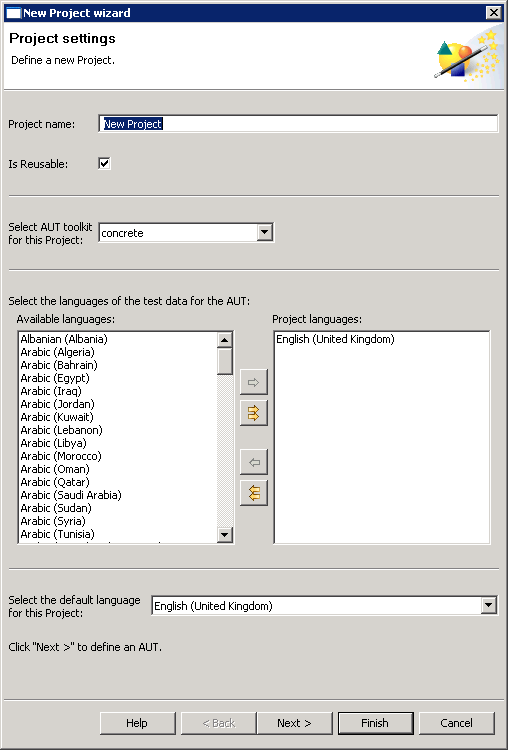
\includegraphics[width=12cm]{Tutorials/PS/TutNewProject}
\caption{New Project Dialog}
\label{TutNewProject}
\end{center}
\end{figure}


\item Leave the \bxname{is reusable} checkbox selected.
\item Choose \bxname{concrete} as the toolkit.
\item Choose \bxcaption{English (United States)} as the \gdproject{} language and select \bxcaption{Next}.
\bxtipp{Your environment language is pre-selected in the \gdproject{} languages list. If this is not \bxname{English (United States)}, remove it from the \gdproject{} languages for now. This first test is monolingual.}
\item A window will appear in which you can define an \gdaut{} (\bxfigref{TutDefineAUT}).

\begin{figure}[h]
\begin{center}
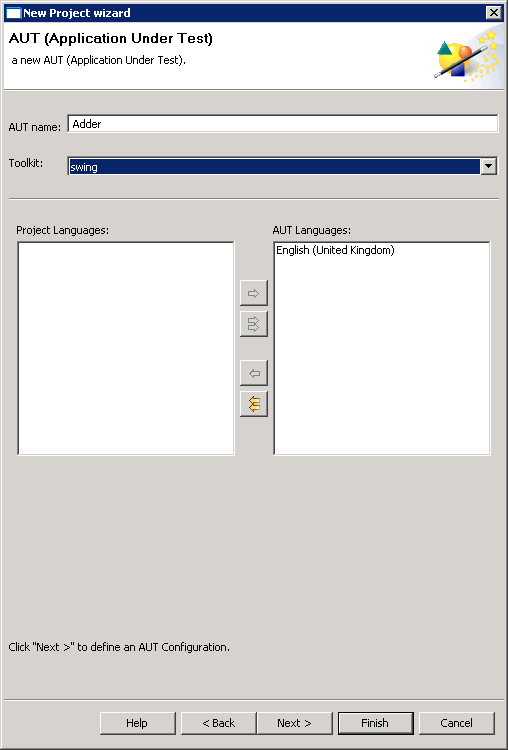
\includegraphics[width=12cm]{Tutorials/PS/TutDefineAUT}
\caption{Define AUT Dialog}
\label{TutDefineAUT}
\end{center}
\end{figure}
 
\item Enter \bxshell{Adder} as the \gdaut{} name. 
\item Choose \bxname{swing} as the toolkit.
\item Select \bxcaption{Next}.
%\item Choose \bxcaption{English} as the \gdaut{} language and select \bxcaption{Next}.
\item In the window which appears (\bxfigref{TutConfigureAUT}) you can create a configuration for this \gdaut{}. 
\item Click the \bxname{basic} button.
\item Leave the default configuration name, which is a composite of the \gdaut{} name, and the \gdserver{} host. 

\begin{figure}[h]
\begin{center}
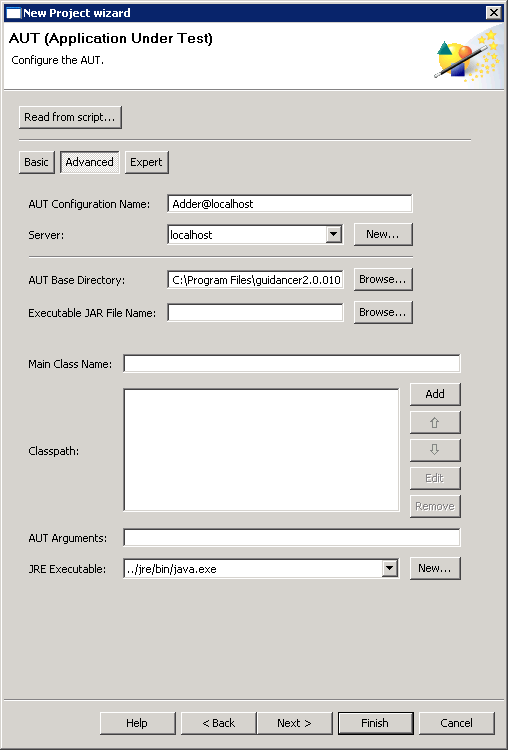
\includegraphics[width=12cm]{Tutorials/PS/TutConfigureAUT}
\caption{\gdaut configuration window}
\label{TutConfigureAUT}
\end{center}
\end{figure}

\item If you started the default \gdserver, choose \bxcaption{localhost} as the \gdserver{} host. If you started a different \gdserver, select \bxcaption{add} and add a new \gdserver \bxpref{serverConfigPrefPage}. 
\item Enter the JAR file name, 
(i.e. \bxshell{C:$\backslash$Program Files$\backslash$GUIdancer$\backslash$aut$\backslash$adder$\backslash$adder.jar}). 
\item Click the \bxcaption{advanced} button.
\item Define the \bxname{Java} runtime location, either by choosing one 
of the available ones from the list, or by adding another. 
(e.g 
\bxshell{C:$\backslash$Program Files$\backslash$Java$\backslash$jre1.6$\backslash$bin$\backslash$javaw.exe}). 

Use the java.exe if you want to use a console, use the javaw.exe if you do not want a console.
\item Select \bxcaption{finish} to create this \gdproject{}. 
\end{enumerate}
